% Aberrations as a piecewise-linear fit of the wavefront (Chapter 5,
% sec:aberrations-as-shifts). After the supervisor's drawing at the
% 2026-11-24 meeting; figure approved 2026-11-25 (departure table).
% Redrawn 2026-11-25 (author): the wavefronts sit on the system diagram;
% polished the same day (larger labels, the fit made to stand out).
% Each panel: an emitter in a heterogeneous sample sends spherical
% wavefronts that are clean near the emitter and distorted after the
% inclusions; behind the objective the wavefront is nominally plane; at the
% lenslets (N = 7 segments) the ideal (dashed), real (thin) and
% piecewise-linear approximated (thick) wavefronts are superimposed. The
% approximation joins the real wavefront at the segment ends, so each
% piece has the segment's mean slope. (a) and (b): two emitters in the same
% sample, with different distortions and fits. Schematic; the distortions
% are made up and enlarged at the lenslets.
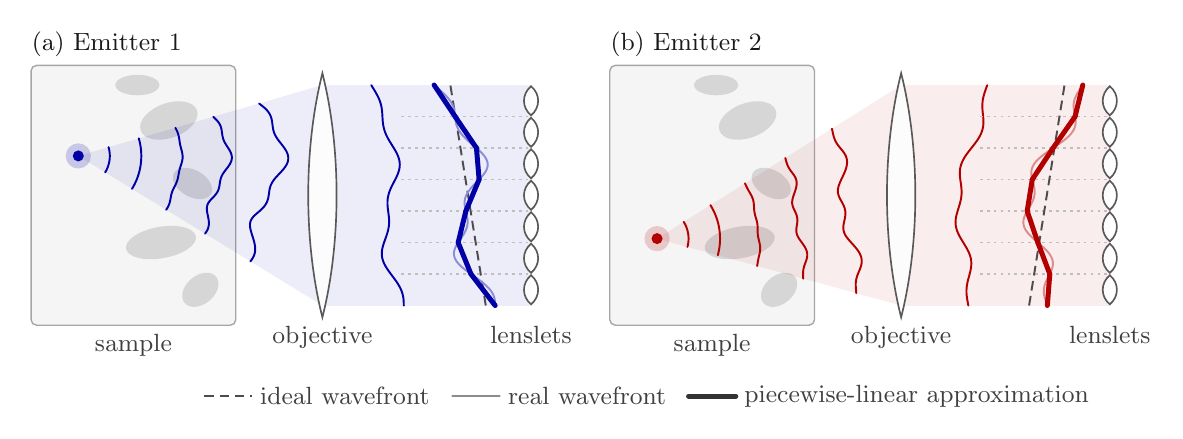
\begin{tikzpicture}[
    x=1cm,y=1cm,
    font=\small,
    lab/.style={font=\small,text=black!75,inner sep=1.5pt,align=center},
    title/.style={font=\small,text=black!90,inner sep=1.5pt},
    ideal/.style={draw=black!70,line width=0.7pt,dash pattern=on 3.5pt off 2pt},
    real/.style={line width=0.7pt,line cap=round,line join=round},
    approx/.style={line width=1.8pt,line cap=round,line join=round},
    lens/.style={draw=black!65,line width=0.6pt,fill=white,fill opacity=0.85}
]
% ---- shared geometry (cm; not to scale) ----
\def\sw{2.6}      % sample width
\def\xe{0.6}      % emitter depth in the sample
\def\xl{3.7}      % objective
\def\hl{1.4}      % half-height of the beam at the objective and the pupil
\def\xm{4.55}     % a wavefront between the objective and the lenslets
\def\xw{5.55}     % the wavefront at the lenslets
\def\xa{6.35}     % lenslet array
\def\s{0.4}       % wavefront displacement per unit of phase
\def\sl{0.75}     % the same at the lenslets, enlarged for visibility
% aberration part of the wavefront, u in [-1,1] across the beam. The last
% term vanishes at the segment ends (u = -1 + 2k/7), so it leaves the fit
% unchanged and bows the real wavefront within each segment.
\def\abA(#1){(0.30*sin(deg(4*(#1)+0.3))+0.12*sin(deg(3.5*pi*((#1)+1))))}
\def\abB(#1){(-0.33*cos(deg(3.5*(#1)))-0.12*sin(deg(3.5*pi*((#1)+1))))}

\foreach \ox/\ye/\tilt/\ab/\c/\title in
    {0/0.5/-0.3/\abA/blue!65!black/{(a) Emitter 1},
     7.35/-0.55/0.3/\abB/red!70!black/{(b) Emitter 2}} {
\begin{scope}[shift={(\ox,0)}]
    % ---- sample and its refractive-index variations ----
    \fill[black!4,rounded corners=2pt] (0,-1.65) rectangle (\sw,1.65);
    \foreach \cx/\cy/\rx/\ry/\ang in {1.75/0.95/0.38/0.22/20, 2.05/0.15/0.27/0.17/-30,
            1.65/-0.6/0.45/0.2/10, 2.15/-1.2/0.26/0.18/40, 1.35/1.4/0.28/0.13/0}
        \fill[black!16,rotate around={\ang:(\cx,\cy)}] (\cx,\cy) ellipse ({\rx} and {\ry});
    \draw[black!35,line width=0.5pt,rounded corners=2pt] (0,-1.65) rectangle (\sw,1.65);
    \node[title,anchor=south west] at (-0.05,1.7) {\title};

    % ---- light: cone to the objective, collimated beam to the lenslets ----
    \fill[\c,opacity=0.07] (\xe,\ye) -- (\xl,\hl) -- (\xl,-\hl) -- cycle;
    \fill[\c,opacity=0.07] (\xl,-\hl) rectangle (\xa,\hl);
    \pgfmathsetmacro{\aT}{atan2(\hl-\ye,\xl-\xe)}
    \pgfmathsetmacro{\aB}{atan2(-\hl-\ye,\xl-\xe)}

    % ---- spherical wavefronts: clean near the emitter, distorted after
    % the inclusions (the distortion grows with the path through them) ----
    \foreach \r/\amp in {0.4/0, 0.8/0, 1.3/0.15, 1.85/0.6, 2.5/1} {
        \draw[\c,real,samples=90,domain=0:1]
            plot ({\xe+(\r+\amp*\s*\ab(2*\x-1))*cos(\aB+\x*(\aT-\aB))},
                  {\ye+(\r+\amp*\s*\ab(2*\x-1))*sin(\aB+\x*(\aT-\aB))});
    }
    \fill[\c,opacity=0.18] (\xe,\ye) circle (0.16);
    \fill[\c] (\xe,\ye) circle (0.07);

    % ---- objective (biconvex) ----
    \draw[lens] (\xl,-1.55) .. controls (\xl+0.24,-0.6) and (\xl+0.24,0.6) .. (\xl,1.55)
                           .. controls (\xl-0.24,0.6) and (\xl-0.24,-0.6) .. cycle;

    % ---- behind the objective: nominally plane, but distorted ----
    \draw[\c,real,samples=90,domain=-1:1]
        plot ({\xm+\s*(\tilt*\x+\ab(\x))},{\hl*\x});

    % ---- at the lenslets: segments, ideal, real, approximation ----
    \foreach \k in {1,...,6}
        \draw[black!25,line width=0.4pt,dash pattern=on 1pt off 1.5pt]
            (\xw-0.85,{-\hl+2*\hl*\k/7}) -- (\xa,{-\hl+2*\hl*\k/7});
    \draw[ideal] ({\xw-\sl*\tilt},-\hl) -- ({\xw+\sl*\tilt},\hl);
    \draw[\c!45,real,samples=140,domain=-1:1]
        plot ({\xw+\sl*(\tilt*\x+\ab(\x))},{\hl*\x});
    \foreach \k in {0,...,6} {
        \pgfmathsetmacro{\ua}{-1+2*\k/7}
        \pgfmathsetmacro{\ub}{-1+2*(\k+1)/7}
        \pgfmathsetmacro{\pa}{\tilt*\ua+\ab(\ua)}
        \pgfmathsetmacro{\pb}{\tilt*\ub+\ab(\ub)}
        \draw[\c,approx] ({\xw+\sl*\pa},{\hl*\ua}) -- ({\xw+\sl*\pb},{\hl*\ub});
    }

    % ---- lenslet array in the back pupil: N = 7 segments ----
    \pgfmathsetmacro{\pw}{2*\hl/7}
    \foreach \k in {0,...,6} {
        \pgfmathsetmacro{\ya}{-\hl+\pw*\k+0.015}
        \pgfmathsetmacro{\yb}{-\hl+\pw*(\k+1)-0.015}
        \draw[lens] (\xa,\ya) .. controls (\xa+0.12,\ya+0.25*\pw) and (\xa+0.12,\yb-0.25*\pw) .. (\xa,\yb)
                             .. controls (\xa-0.12,\yb-0.25*\pw) and (\xa-0.12,\ya+0.25*\pw) .. cycle;
    }

    % ---- labels ----
    \node[lab,anchor=north] at (\sw/2,-1.7) {sample};
    \node[lab,anchor=north] at (\xl,-1.6) {objective};
    \node[lab,anchor=north] at (\xa,-1.6) {lenslets};
\end{scope}
}
% ---- legend ----
\begin{scope}[shift={(2.2,-2.55)}]
    \draw[ideal] (0,0) -- (0.6,0);
    \node[lab,anchor=west] at (0.65,0) {ideal wavefront};
    \draw[black!45,real] (3.15,0) -- (3.75,0);
    \node[lab,anchor=west] at (3.8,0) {real wavefront};
    \draw[black!80,approx] (6.15,0) -- (6.75,0);
    \node[lab,anchor=west] at (6.8,0) {piecewise-linear approximation};
\end{scope}
\end{tikzpicture}
